\subsection{Установка цен поставщика}
\subsubsection{Описание изменений ,,Установка цен поставщика``}
\begin{itemize}	
	\item В конфигурацию добавлен новый   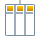
\includegraphics[width=0.02\linewidth]{images/sp} справочник ,,Типы цен номенклатуры контрагентов''. В этом справочнике будут храниться цены контрагентов, их наименование и тип. Справочник подчинен справочнику ,,Контрагенты'' и доступен из формы элемента справочника ,,Контрагенты'' по кнопке 	
\includegraphics[width=0.02\linewidth]{images/mv} ,,Перейти''
	\sidenote[-2ex][]{Переход из меню не доступен}
%\sidenote[-2ex][]{A note}
    Рис.~\ref{ris:14.jpg}	
	\begin{figure}[H]
		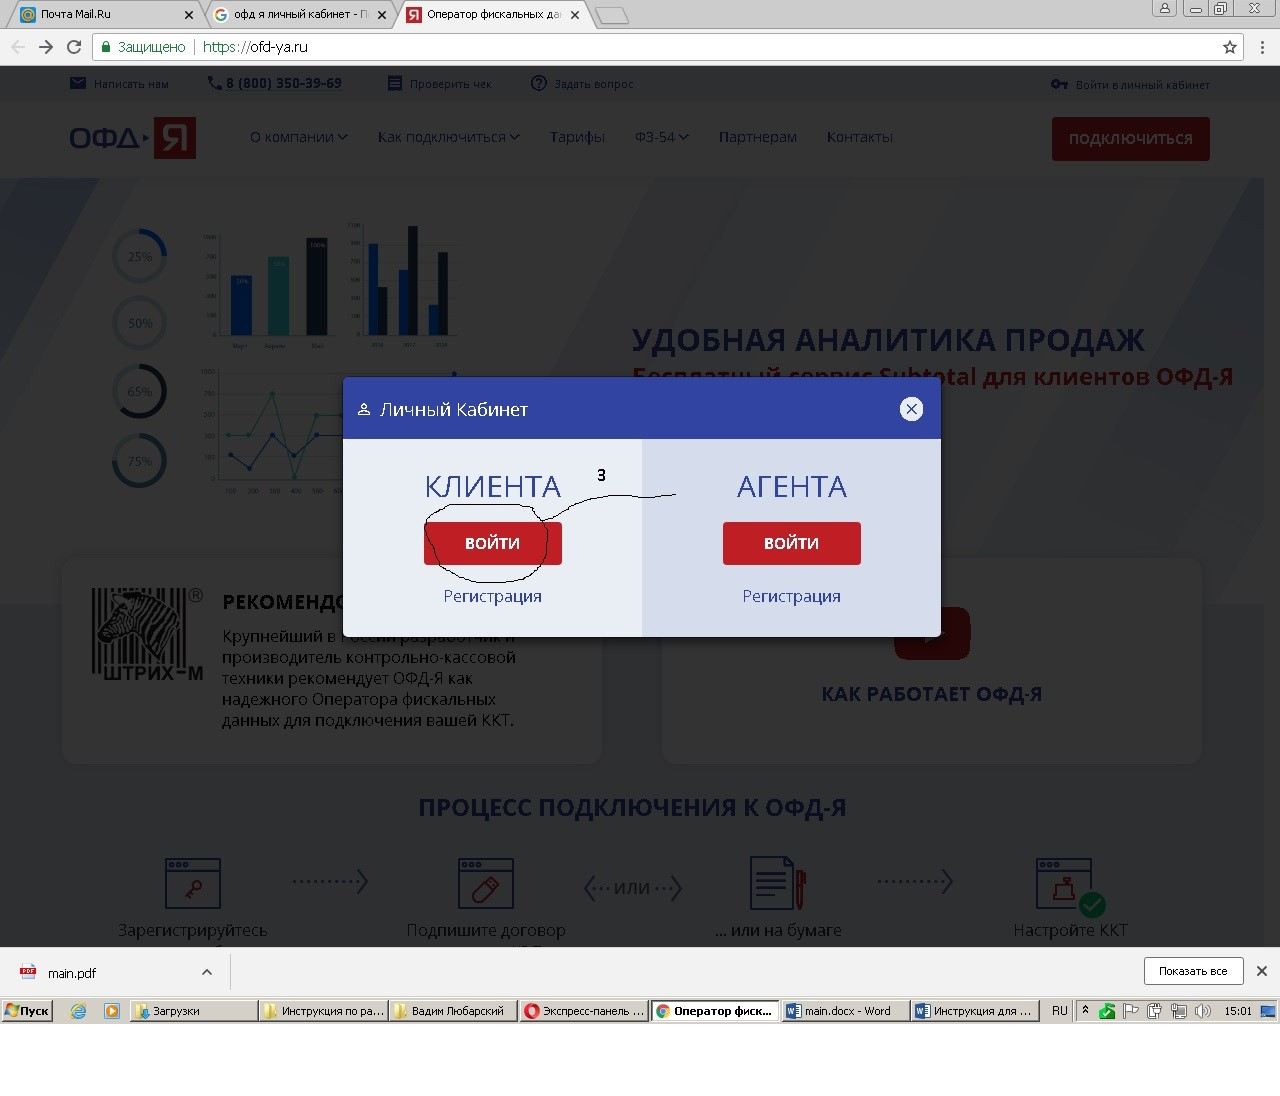
\includegraphics[width=0.8\textwidth]{14.jpg}
		\caption{Где справочник "<Типы цен номенклатуры контрагентов">.}
		\label{ris:14.jpg}
	\end{figure}
	\item Для добавления типа по конкретному поставщику, нужно из "<карточки"> контрагента открыть справочник "<Типы цен номенклатуры контрагентов"> как указано на Рис.~\ref{ris:14.jpg}
  	\item И с помощью кнопки \keys{Создать}  Добавить новый элемент
    Рис.~\ref{ris:15.jpg}	
  	\begin{figure}[H]
  		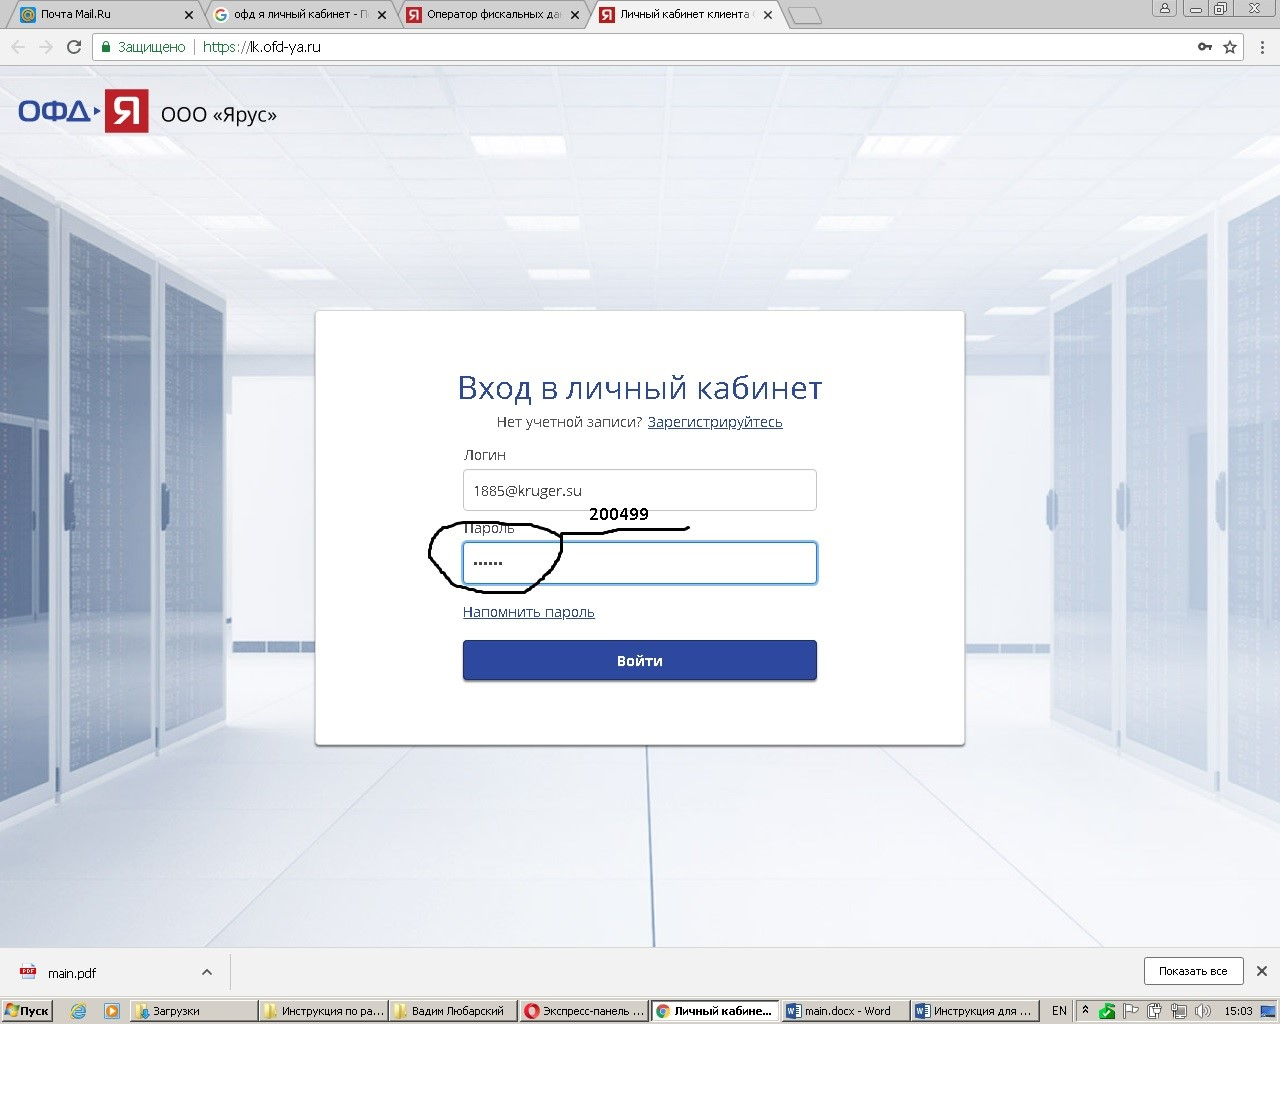
\includegraphics[width=0.7\textwidth]{15.jpg}
  		\caption{Создание нового элемента.}
  		\label{ris:15.jpg}
  	\end{figure}
	\item Откроется форма создания нового элемента справочника "<Типы цен номенклатуры контрагентов"> Рис.~\ref{ris:16.jpg}
	\begin{figure}[H]
		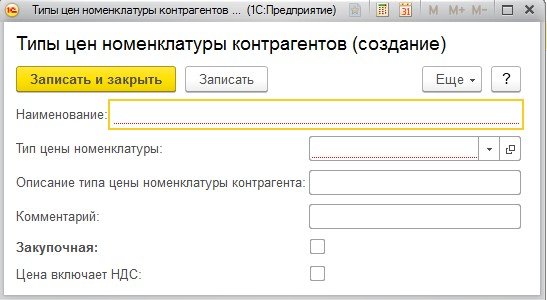
\includegraphics[width=0.7\textwidth]{16.jpg}
		\caption{Новый элемент справочника.}
		\label{ris:16.jpg}
	\end{figure}  
  
	\item Необходимо заполнить данные для создания нового элемента справочника "<Типы цен номенклатуры контрагентов"> и  сохранить используя кнопку \keys{Записать и закрыть}  Рис.~\ref{ris:17.jpg}
	\item Если тип создаваемой цены \textbf{"<Закупочная">} т.е. эта цена будет подставляться в документ ,,Поступление товаров'', то необходимо поставить "<галочку"> у реквизита ,,Закупочная''. \par 
	\textbf{Внимание!!!} у контрагента может быть только одна цена с признаком ,,Закупочная''. 
  	\begin{figure}[H]
  		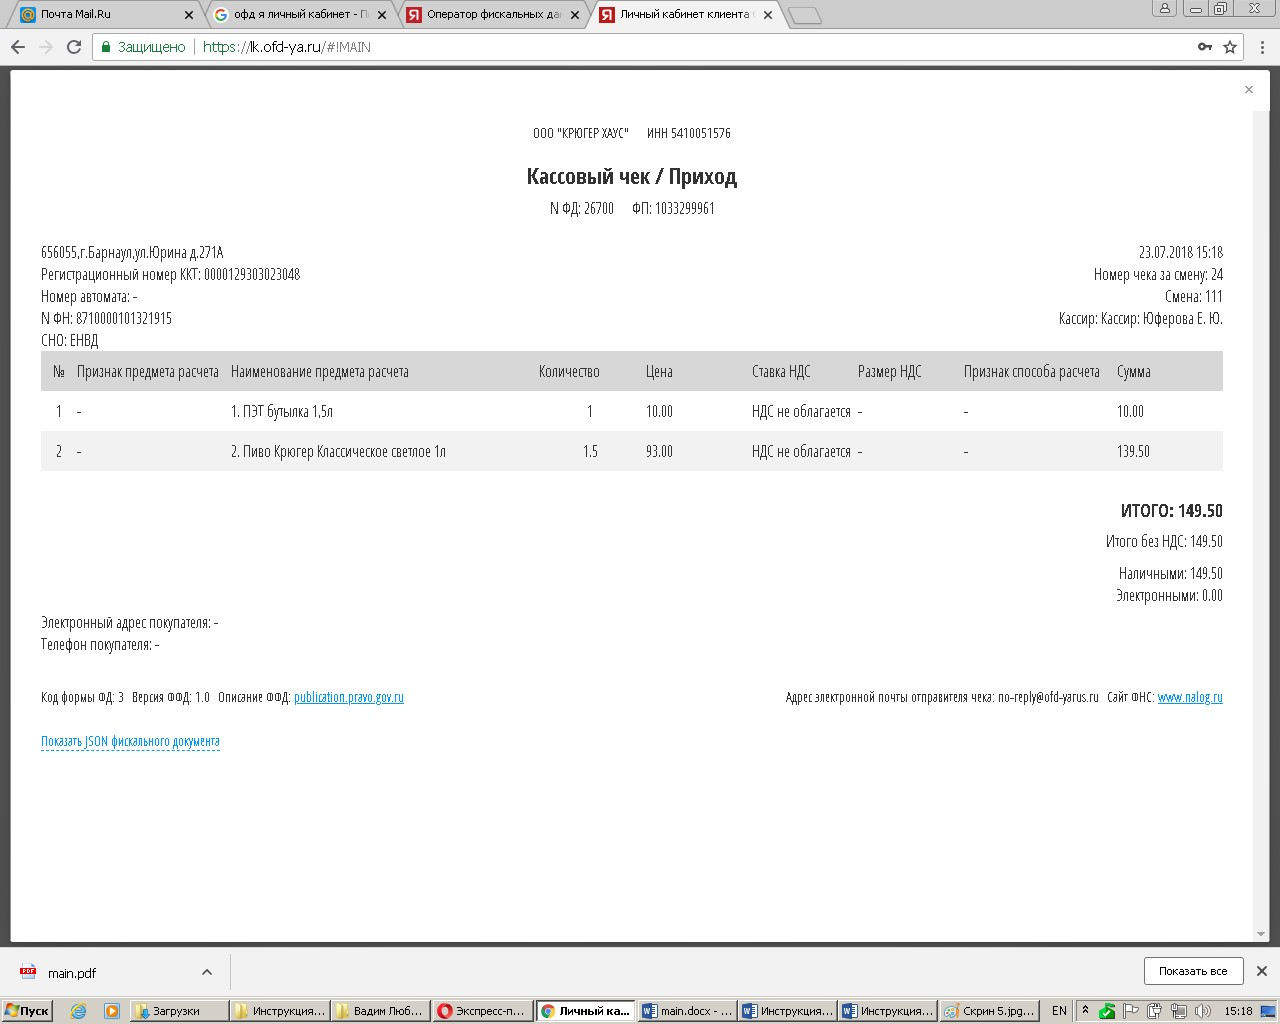
\includegraphics[width=0.7\textwidth]{17.jpg}
  		\caption{Заполненные данные.}
  		\label{ris:17.jpg}
  	\end{figure}  
  
  	\item Появилась цена поставщика.  Рис.~\ref{ris:18.jpg}
  	Повторяем процедуру добавления, столько раз сколько цен у данного поставщика.
  \begin{figure}[H]
  	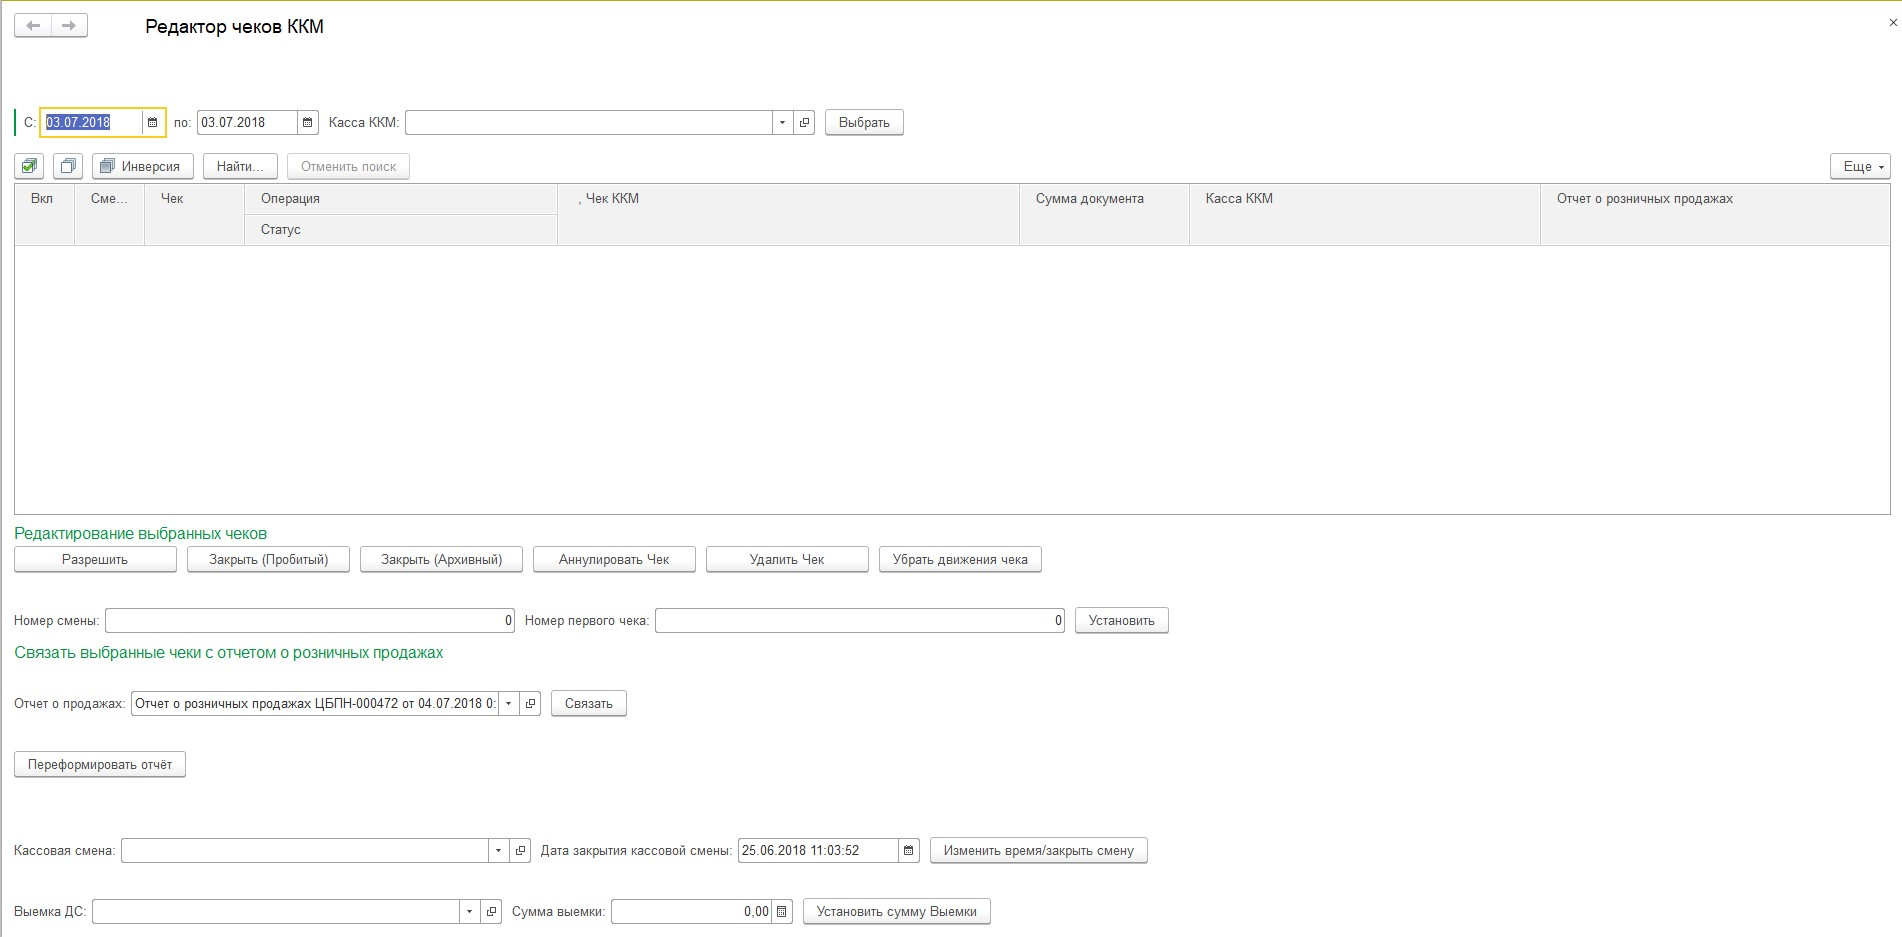
\includegraphics[width=0.7\textwidth]{18.jpg}
  	\caption{Добавлена цена.}
  	\label{ris:18.jpg}
  \end{figure}  
  
  
  
\end{itemize}

%	\begin{figure}[H]
%		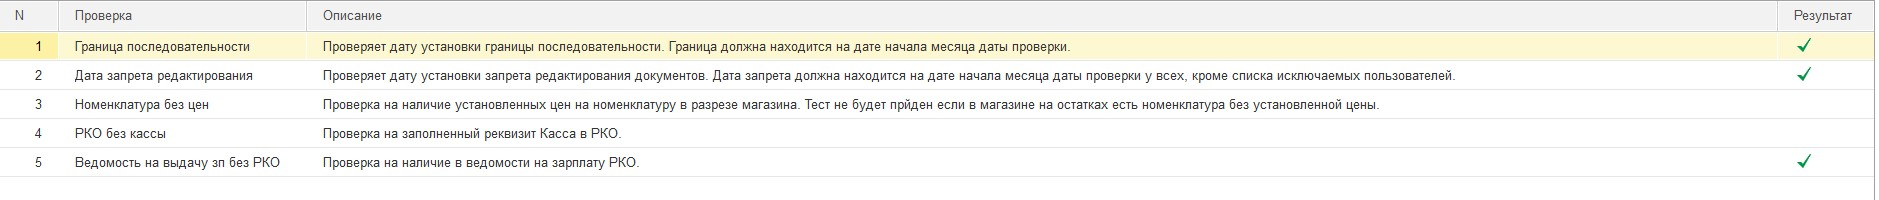
\includegraphics[width=0.8\textwidth]{2.jpg}
%		\caption{Выбор значения.}
%		\label{ris:2.jpg}
%	\end{figure}
%	Выбрав нужное значение нужно воспользоваться кнопкой ,,Записать`` или  ,,Записать закрыть`` для сохранения изменений Рис.~\ref{ris:3.jpg}
%	\begin{figure}[H]
%		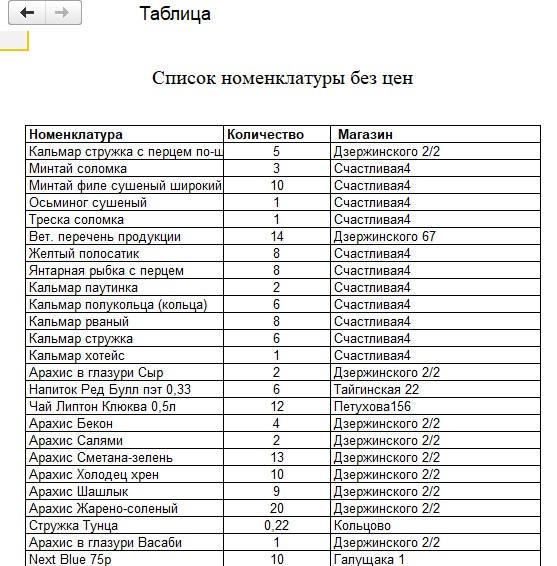
\includegraphics[width=0.8\textwidth]{3.jpg}
%		\caption{Сохранить изменения.}
%		\label{ris:3.jpg}
%	\end{figure}
%	\item После того как в элементы номенклатуры были добавлены значения  ,,Групп номенклатуры`` появляется возможность формирования отчетов с их использованием
%
